\chapter{Infografiche}
\label{cap:studio_infografiche}
\intro{In questo capitolo verranno esaminate le caratteristiche funzionali e di design delle infografiche e 
presentate le loro applicazioni. Verrà inoltre fornita una classificazione delle infografiche basata sulla 
loro struttura e output visivo.}\\

\section{Definizione e applicazioni}
\subsection{Cos'è un infografica e in cosa si distingue dalla data visualization}
%cap1: Design della mente – infografica e data viz” di Paolo Bottazini, Michele Gotuzzo 
Analogamente alla \gls{datavizg}, le infografiche si occupano di rappresentare visivamente i dati al fine di comunicarli in maniera più semplice e accessibile.
Esse trasformano i dati in idee chiare, permettendo di inquadrare facilmente un fenomeno, una situazione o un processo, coadiuvando così la presa di decisioni ponderate sul tema presentato.
Queste idee sono generate a partire dall'interpretazione, formalizzazione e contestualizzazione dei dati, che spesso sono disomogenei per formato, tipo di contenuto e origine. Tale interpretazione ha il compito di 
svelare il significato nascosto nel \emph{dataset} e selezionare le connessioni o fenomeni più interessanti per il destinatario della comunicazione.
In altre parole, l'infografica non si limita a mostrare i dati, ma li organizza e li presenta in un modo da renderne più evidente significato e importanza.

Per raggiungere questo obiettivo, le infografiche combinano elementi testuali e grafici per presentare le informazioni; usando le parole di E. Tufte ``un'infografica mostra visivamente grandezze misurate mediante 
l'uso combinato di punti, linee, un sistema di coordinate, numeri, simboli, parole, ombreggiature e colore''. Pertanto, le infografiche rigettano la tradizione di ``purezza grafica'' (i.e. rappresentazione dei dati 
basata solo su grafici, diagrammi e mappe) imposta alla \gls{datavizg} e abbracciano, invece, un insieme molto più amplio di tecniche di comunicazione visiva, come illustrazioni, immagini, etc.
% TODO: aggiungere citazione come footnote The visual display of quantitative information, Edward Tufte [2001], Introduction, p.10
Inoltre, il focus dell'infografica non è solamente l'oggetto da rappresentare, come invece accade con la \gls{datavizg}. Infatti, le infografiche
prendono in considerazione anche il destinatario della comunicazione, scegliendo e disponendo gli elementi per costruire una narrazione.
Possiamo infatti pensare all'infografica come a una forma di racconto, di lettura che non è di per sé né imparziale né completa, ma si limita a fare luce ed esporre i punti salienti individuati nel \emph{dataset}.
%intro: “L'arte funzionale – Infografica e visualizzazione delle informazioni” di Alberto Cairo
In realtà, tale caratteristica delle infografiche è proprio ciò che maggiormente le distingue dalla \gls{datavizg}. Infatti, mentre le prime sono progettate per presentare i dati raccontandoli attraverso storie specifiche, guidando il lettore con una narrazione, la seconda
è più orientata verso l'esplorazione autonoma delle informazioni da parte del fruitore, che deve analizzare e scoprire i dati per conto proprio. 
Questa differenza nel livello di analisi richiesto si ripercuote anche sul tipo di pubblico di ciascun tipo di rappresentazione. Nello specifico, le infografiche, grazie alla loro capacità di semplificare e contestualizzare i dati, sono accessibili anche a coloro
che non possiedono capacità analitiche avanzate e, pertanto, hanno un pubblico più ampio. 

%intro: “L'arte funzionale – Infografica e visualizzazione delle informazioni” di Alberto Cairo
Nonostante queste differenze, infografiche e \gls{datavizg} sono strettamente connesse e complementari. Le infografiche, pur essendo maggiormente orientate alla narrazione, 
possono includere elementi che stimolano l'esplorazione autonoma dei dati. Allo stesso modo, le \emph{visualizzazioni dei dati} possono contenere aspetti narrativi che facilitano 
l'interpretazione.


\subsection{Applicazioni e vantaggi}
Le infografiche sono strumenti versatili che vengono utilizzati in una vasta gamma di settori e contesti, in particolare al fine 
di analizzare o presentare dati. Offrono infatti vantaggi significativi che le rendono particolarmente adatte a questi scopi.

%Infographics: The New Communication Tools in Digital Age, Waralak V. Siricharoen
Per quanto riguarda l'\textbf{analisi dei dati}, le infografiche sono utili per la cosiddetta \gls{expdataanalysisg}, dove il fruitore non ha una domanda precisa a cui sta cercando risposta, bensì 
vuole semplicemente scoprire cosa emerge di interessante dal \emph{dataset}.

Per quanto riguarda invece la \textbf{presentazione dei dati}, va da sé che le infografiche siano perfette per tale scopo, in quanto riescono attraverso una narrazione a comunicare in maniera efficace 
e abbracciare in tal modo un pubblico molto amplio.

\bigskip
\noindent In generale, quale sia l'applicazione, l'uso di infografiche consente anche di:
\begin{itemize}
    \item \textbf{Facilitare la scoperta di informazioni} nascoste e \textbf{stimolare la curiosità} per una ricerca futura;
    \item \textbf{Semplificare la comprensione}, facilitando così il raggiungimento della \emph{saggezza};
    \item \textbf{Raccontare una storia} che permetta una visione d'insieme della situazione, fenomeno o processo presentato.
\end{itemize}



\section{Classificare le infografiche}
\subsection{Metodi di classificazione}\label{subsec:info_classifica}
% file criteri_scelta_infografica_v0.1.0
Una prima classificazione delle infografiche può essere fatta \textbf{in base all'output visivo}. Nello specifico, si hanno:
\begin{itemize}
    \item \textbf{Infografiche statiche}, in cui le informazioni sono rappresentate e visibili tutte in un'unica volta, avendo così un impatto più
    veloce e immediato sul pubblico.
    \begin{itemize}
        \item Esempio: infografiche presenti nei giornali.
    \end{itemize}
    \item \textbf{Infografiche animate}, in cui le informazioni sono presentate sequenzialmente in maniera consistente oppure contengono altri tipi di animazione.
    \begin{itemize}
        \item Esempio: infografiche realizzate tramite presentazioni multimediali.
    \end{itemize}
    \item \textbf{Infografiche interattive}, in cui le informazioni sono presentate in base a scelte operate dall'utente.
    \begin{itemize}
        \item Esempio: infografiche online in cui è l'utente a selezionare il dettaglio a partire da un insieme complesso di informazioni visualizzate.
    \end{itemize}
\end{itemize}

\bigskip
\noindent Un'altra classificazione può essere fatta \textbf{in base all'obiettivo}. Nello specifico, si hanno:
\begin{itemize}
    \item \textbf{Infografiche basate su processi ordinati}, le quali vengono usate per mostrare passo dopo passo un processo o una 
    sequenza ordinata di informazioni ad esempio per insegnare qualcosa di nuovo all'utente (e.g. ricette).
    \item \textbf{Infografiche a mo' di lista}, in questo caso le informazioni sono rappresentate sotto forma di elenco testuale, eventualmente accompagnato da icone.
    Per costruzione, queste infografiche permettono di mostrare molte informazioni e, allo stesso tempo, di farle comprenderle velocemente.
    \item \textbf{Infografiche basate sul tempo}, in cui viene mostrata una sequenza cronologica di eventi, in altre parole come si evolve una storia o un soggetto nel tempo.
    Quest'ultimo è solitamente rappresentato tramite una linea, chiamata appunto ``linea del tempo''.
    \item \textbf{Infografiche basate sul confronto}, esse comparano due diversi argomenti in contrasto ponendoli uno a fianco all'altro.  Ciò ritorna molto utile per mostrare
    quali elementi i due hanno in comune oppure per quanto divergono o sono superiori/inferiori uno rispetto all'altro.
    \item \textbf{Infografiche basate su una gerarchia}, le quali vengono utilizzate per mostrare informazioni organizzate per livelli e il collegamento tra questi.
    \item \textbf{Infografiche basate su informazioni correlate poste allo stesso livello}, in cui si vuole comunicare un nuovo concetto o dare una panoramica su un argomento; infatti,
    tali infografiche sono anche dette ``Infografiche informative''. Solitamente, lo spazio viene diviso in sezioni con un proprio titolo descrittivo.
\end{itemize}


\subsection{Infographic-helper}
Come accennato in precedenza, l'infografica è una forma di racconto e, pertanto, la scelta e scrittura della storia da comunicare sono centrali nella sua costruzione.
Nel corso dello stage si è dunque voluto sviluppare uno strumento prototipale, \emph{Infographic-helper}, che potesse aiutare il ``narratore'' in tale compito.
Nello specifico, questo strumento consente di validare tale narrativa, oltre a individuarne le parti e l'obiettivo principale.

Lo strumento è disponibile a \href{http://www.overleaf.com}{questo link}.

\subsubsection{Validazione della narrativa}
Uno degli obiettivi di \emph{Infographic-helper} è garantire che la narrativa dell'infografica sia persuasiva e venga recepita efficacemente dal pubblico. 
Questi obiettivi coincidono con quelli della retorica, la quale fornisce i principi per costruire messaggi convincenti e chiari, che espongono il punto di vista del comunicatore in maniera comprensibile. 
Questi principi non solo sono applicabili alla pura comunicazione verbale, ma si rivelano utili anche per le infografiche. 
Infatti, nonostante queste siano rappresentazioni visive, esse sono comunque una forma di narrazione e comunicazione e pertanto oggetto di retorica. 

Aristotele, pioniere di quest'arte, definisce suddetti principi come \emph{ethos}, \emph{pathos} e \emph{logos}. Nello specifico:
\begin{itemize}
    \item \textbf{\emph{Ethos}}, comprende tutto ciò che stabilisce o aumenta la credibilità e autorità del comunicatore e delle fonti;
    \item \textbf{\emph{Pathos}}, comprende tutto ciò che suscita emozioni nel pubblico, che crea una connessione emotiva con gli spettatori;
    \item \textbf{\emph{Logos}}, comprende tutto ciò che fa parte di un'argomentazione razionale, logica e coerente, come dati e statistiche.
\end{itemize}
\emph{Infographic-helper} si ispira dunque a questi principi aristotelici per migliorare la costruzione delle storie delle infografiche. Nello specifico, controlla che questi elementi siano presenti
nel testo e, eventualmente, ne suggerisce di altri.

In aggiunta a questi elementi retorici, \emph{Infographic-helper} tiene conto anche del target dell'infografica, ovvero il pubblico a cui è destinata, per poter contestualizzare meglio la storia. 
Inoltre, lo strumento controlla anche se sono presenti eventuali elementi estranei o irrilevanti per il tema principale della storia. 

\bigskip
\noindent Queste funzionalità sono implementate attraverso interrogazione a un \gls{llm}, nello specifico si utilizza il modello \textbf{\gls{llama7bg}} attraverso \textbf{\gls{llamacppg}}, reso disponibile dall'azienda ospitante.

Il \emph{prompt} utilizzato è il seguente:
\begin{lstlisting}[style=htmlcssjs]
Questa è una conversazione tra User e Llama, un chatbot amichevole. Llama è disponibile, onesto, bravo a scrivere e non manca mai di rispondere immediatamente e con precisione a qualsiasi richiesta.

User: 
Devo presentare il seguente testo a ${target}.
${ethos}.

Testo:
${storia}

Domande:
1.	Supponi che un elemento è di 'pathos' se può indurre il pubblico a sentire (o non sentire) una connessione emotiva con il contenuto.
    Riporta tutti gli elementi (frasi, espressioni e parole) di 'pathos' del Testo, SOLO se hanno senso nel contesto del Testo. Suggerisci altre frasi incisive di 'pathos' da poter inserire nel Testo.
2.  Supponi che un elemento è di 'ethos' se può indurre il pubblico a ritenere che l'autore sia (o meno) affidabile e credibile.
    Riporta tutti gli elementi (frasi, espressioni e parole) di 'ethos' del Testo, SOLO se hanno senso nel contesto del Testo. Suggerisci altre frasi incisive di 'ethos' da poter inserire nel Testo basandoti sul mio ruolo SE rilevante al tema del Testo.
3.  Supponi che un elemento è di 'logos' se può indurre il pubblico a credere che l'argomentazione sia (o meno) logica e supportata da prove adeguate.
    Riporta tutti gli elementi (frasi, espressioni e parole) di 'logos' del Testo, SOLO se hanno senso nel contesto del Testo. Suggerisci altre frasi incisive di 'logos' da poter inserire nel Testo.
4.	Supponi che un elemento è 'estraneo' se può ritenersi estraneo rispetto al tema principale del Testo oppure può ritenersi un'assurdità.
    Riporta tutti gli elementi (frasi, espressioni e parole) 'estraneo' presenti nel Testo.

[...continua...]
\end{lstlisting}
% TODO: inserire modello usato corretto (7b?) e llama.cpp
dove \texttt{\$target} rappresenta il pubblico di destinazione dell'infografica e \texttt{\$ethos} rappresenta il ruolo di chi espone la storia, inseriti per una maggiore contestualizzazione della storia poi riportata (inserita al posto di \texttt{{\$storia}}).

\subsubsection{Ricerca del layout da utilizzare}
L'altro obiettivo di \emph{Infographic-helper} è quello di classificare la storia in base alla seconda classificazione data in \ref{subsec:info_classifica} (ovvero la ``classificazione per obiettivo'') e trovare le sue principali parti costitutive.
Tali informazioni consentono di individuare il \emph{layout} più adatto per raccontare visivamente la storia e definire l'argomento specifico da trattare per ciascuna delle sezioni di tale \emph{layout}.

I possibili \emph{layout} sono descritti al paragrafo \ref{subsec:info_layout}.

\bigskip
\noindent Queste funzionalità sono anch'esse implementate attraverso interrogazione al \gls{llm} descritto precedentemente. 

Il \emph{prompt} utilizzato è il seguente:
\begin{lstlisting}[style=htmlcssjs]
[...segue...]
5.	Quali sono le parti in cui si divide il testo? Per ogni parte, dimmi solo un titoletto breve.
6.	Tolta l'introduzione, identifica la relazione generale tra le parti come una delle seguenti:
    -	parti di una lista, 
    -	parti di una linea del tempo, 
    -	parti poste a confronto, 
    -	parti che compongono gerarchia, 
    -	parti correlate poste allo stesso livello, 
    -	parti di un processo ordinato. 

Fornisci solamente le risposte nel seguente formato JSON: 
{ 'pathos': { 'presente': boolean, 'elementi': [string], 'suggerimenti': [string] }, 'ethos': { 'presente': boolean, 'elementi': [string], 'suggerimenti': [string] }, 'logos': { 'presente': boolean, 'elementi': [string], 'suggerimenti': [string] }, 'elementi_estraneo': {'presente': boolean, 'elementi': [string]}, 'parti': [string], 'relazione': 'string' }


Llama:
\end{lstlisting}

\noindent Si noti inoltre che è stata definita una \gls{grammaticag} corrispondente allo schema menzionato nel prompt (fornito per ulteriore chiarezza), la quale consente di ottenere l'output del \gls{llm} nel formato fisso \gls{jsong} indicato. 
Questo approccio facilita il \emph{parsing} dei dati, garantendo risposte precise con un formato standard, e ne agevola l'eventuale integrazione futura con un'interfaccia grafica.


\subsubsection{Limitazioni dello strumento}
Come già accennato precedentemente \emph{Infographic-helper} è uno strumento prototipale, presenta infatti diverse limitazioni.
Innanzitutto, l'applicativo è disponibile soltanto da riga di comando e non dispone di un'interfaccia grafica.
Inoltre, esso non ha la capacità di individuare molteplici obiettivi. Potrebbero essere infatti presenti diverse macro-sezioni nella narrativa
con obiettivi distinti. 
Lo strumento, inoltre, non è capace di valutare la veridicità del contenuto della storia, ma valida soltanto il modo in cui questo è comunicato. Pertanto, è compito del'utente
assicurarsi che quanto scritto corrisponda a verità.

Ciononostante, \emph{Infographic-helper} ha il potenziale per essere migliorato e offrire un'esperienza utente più semplice e intuitiva.
%TODO: aggiungere che fa schifo ?, aggiungere parti test ?



\section{Design delle infografiche}
\subsection{I fattori che influenzano il design}
Possiamo ordinare gerarchicamente i fattori che influenzano, in generale, la presentazione dei dati. Tale gerarchia è suddivisa in quattro livelli come segue:
%TODO: inserire immagine, inserire da dove presa immagine, spiegare come funziona l'immagine (o aggiungi leggenda nell'immagine)
\begin{figure}[H] 
    \centering 
    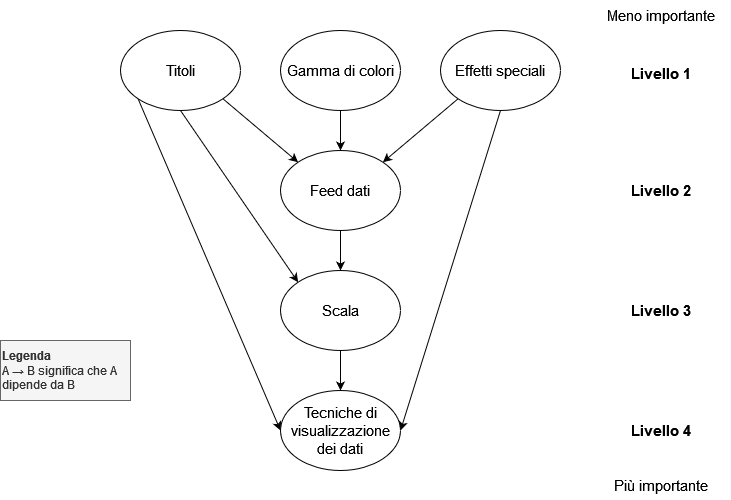
\includegraphics[width=0.8\columnwidth]{infografiche/fattori_design_info.png} 
    \caption{Gerarchia dei fattori che influenzano la presentazione dei dati}
    \label{fig:fattori_design_info}
\end{figure}
Vediamo dunque come applicare al meglio tali fattori nella costruzione del design di un'infografica.

\subsubsection{I titoli}
Le intestazioni devono essere incisive e invogliare il fruitore dell'infografica a continuare a visionare la presentazione. 
A tal fine, i titoli sono generalmente formulati in uno dei seguenti modi:
\begin{itemize}
    \item \textbf{Sotto forma di domanda}, si pone un interrogativo curioso o interessante che stimoli il lettore a cercarne la risposta nei dati presentati.
    \item \textbf{Includendo la statistica principale}, evidenziando il dato presentato più significativo.
    \item \textbf{Come confronto}, si mette in relazione fin da subito due o più elementi di cui se ne mostreranno differenze e similitudini.
    \item \textbf{Come introduzione a un elenco numerato}, il titolo funziona come introduzione a una lista (e.g. ``Top X'').
\end{itemize}

\bigskip
%“Design della mente – infografica e data viz” di Paolo Bottazini, Michele Gotuzzo
%CAP 17: I caratteri
\noindent Un altro elemento fondamentale per quanto riguarda i titoli, e in generale per tutto il testo contenuto nell'infografica, è la scelta del carattere tipografico. 
Nello specifico, la gamma di caratteri utilizzati non deve essere troppo amplia (max. 3 o 4); bisogna invece concentrarsi sulla scelta del tipo di carattere, il quale
può avere un impatto significativo sul design complessivo dell'infografica.

A tal fine, si possono applicare le seguenti regole:
\begin{itemize}
    \item Per quanto riguarda l'uso di \textbf{caratteri graziati} (\emph{serif}), essi sono da utilizzare quando si vuole conferire serietà e autorevolezza al testo; sono infatti impiegati tipicamente in saggi e quotidiani. 
    Tuttavia, possono risultare meno leggibili su schermo.
    \begin{itemize}
        \item Esempio: Times New Roman.
    \end{itemize}
    \item Per quanto riguarda l'uso di \textbf{caratteri senza grazie} (\emph{sans serif}), essi sono da utilizzare per testi brevi e/o su schermi, in quanto più leggibili.
    \begin{itemize}
        \item Esempio: Arial (adatto per testi lunghi, essendo più stretto), Verdana (ideale per frasi ad effetto), Helvetica.
    \end{itemize}
    \item Per quanto riguarda l'uso di \textbf{caratteri decorativi}, essi sono spesso difficili da utilizzare e generalmente, dunque, sono da evitare. Possono essere considerati, seppur con prudenza, per casi specifici per riflettere il tema discusso nella presentazione.
    \begin{itemize}
        \item Esempio: caratteri calligrafici o fumettistici.
    \end{itemize}
    \item Per quanto riguarda l'uso del \textbf{grassetto} (\emph{bold}), è da utilizzare per evidenziare componenti testuali brevi e focalizzare l'attenzione su di essi. 
    \item Per quanto riguarda l'uso del \textbf{corsivo} (\emph{italic}), è da utilizzare per citazioni o termini particolari.
    \item Per quanto riguarda l'uso del \textbf{maiuscolo}, è da utilizzare per dare maggiore importanza o evidenziare testi brevi, come i titoli, in quanto corrisponde ad un ``innalzamento della voce''.
\end{itemize}
Sempre con riferimento ai caratteri, è importante seguire anche le seguenti regole:
\begin{itemize}
    \item Per quanto riguarda la \textbf{sottolineatura}, nel web questa è da evitare per evidenziare elementi (preferendo invece il grassetto), in quanto solitamente rappresenta un collegamento 
    ipertestuale.
    \item Per quanto riguarda l'\textbf{interlinea}, conviene che la distanza tra una riga e l'altra sia abbastanza ampia da consentire una lettura agevole.
    \item Per quanto riguarda l'\textbf{allineamento}, si utilizza solitamente il ``centrato'' per i titoli, specie se non accompagnati da ulteriore testo. Per il resto, si preferisce invece l'allineamento
    ``a sinistra''.
    \item Per quanto riguarda la \textbf{lunghezza}, testi troppo lunghi non sono letti volentieri dal pubblico e, inoltre, necessiterebbero di caratteri più piccoli, meno leggibili.
\end{itemize}


\subsubsection{I colori}
%“Design della mente – infografica e data viz” di Paolo Bottazini, Michele Gotuzzo
%CAP 16: Il colore
Il colore è un elemento cruciale nel design delle infografiche e, pertanto, è da utilizzare con cura. 
Esso infatti, se scelto in maniera appropriata, può migliorare la leggibilità e facilitare la comprensione e memorizzazione dell'informazione.

Generalmente, si utilizza il colore per catturare l'attenzione, evidenziare dati specifici e per rafforzare il messaggio narrativo. Quest'ultimo punto è possibile in quanto ogni colore porta con sé un 
significato simbolico influenzato dalla cultura e dalla geografia che rende possibile evocare sensazioni e valori specifici nel pubblico.
Di seguito sono riportati i valori più spesso associati ai colori, con riferimento alla cultura dell'Occidente:
\begin{itemize}
    \item Colori caldi:
    \begin{itemize}
        \item \textbf{Rosso}:
        \begin{itemize}
            \item Valori: emozioni forti come amore o aggressività.
            \item In linea con tali valori, viene utilizzato principalmente per attirare l'attenzione.
        \end{itemize}
        \item \textbf{Arancione}:
        \begin{itemize}
            \item Valori: ottimismo, vitalità.
            \item In linea con tali valori, viene generalmente utilizzato per temi giovanili e/o dinamici.
        \end{itemize}
        \item \textbf{Giallo}:
        \begin{itemize}
            \item Valori: energia, allegria, felicità.
            \item In linea con tali valori, viene anch'esso utilizzato principalmente per attirare l'attenzione, specie per temi innovativi.
        \end{itemize}
    \end{itemize}
    \item Colori freddi:
    \begin{itemize}
        \item \textbf{Verde}:
        \begin{itemize}
            \item Valori: salute, natura, tranquillità.
            \item In linea con tali valori, viene generalmente utilizzato per temi riguardanti la sanità, salute ed ecologia.
        \end{itemize}
        \item \textbf{Blu}:
        \begin{itemize}
            \item Valori: affidabilità, sicurezza, stabilità.
            \item In linea con tali valori, viene utilizzato ad esempio da banche o compagnie assicurative.
        \end{itemize}
        \item \textbf{Viola}:
        \begin{itemize}
            \item Valori: eleganza, nobiltà, spiritualità.
            \item In linea con tali valori, viene generalmente utilizzato per temi riguardanti il settore della bellezza o del lusso.
        \end{itemize}
    \end{itemize}
    \item Colori neutri:
    \begin{itemize}
        \item \textbf{Marrone}:
        \begin{itemize}
            \item Valori: terra, calore.
            \item In linea con tali valori, viene generalmente utilizzato per temi riguardanti la natura.
        \end{itemize}
        \item \textbf{Bianco}:
        \begin{itemize}
            \item Valori: purezza, pulizia, semplicità.
            \item In linea con tali valori, viene generalmente utilizzato per temi riguardanti la sanità.
        \end{itemize}
        \item \textbf{Nero}:
        \begin{itemize}
            \item Valori: ribellione, formalità, potenza.
            \item In linea con tali valori, viene generalmente utilizzato per temi di protesta o riguardanti il settore del lusso.
        \end{itemize}
        \item \textbf{Grigio}:
        \begin{itemize}
            \item Valori: modernità, raffinatezza.
            \item In linea con tali valori, viene generalmente utilizzati per temi riguardanti tecnologia o moda.
        \end{itemize}
    \end{itemize}
\end{itemize}

\bigskip
\noindent In ogni caso, è fondamentale mantenere un tono di colore coerente nell'infografica, preferibilmente sobrio. Tuttavia, potrebbe essere utile utilizzare colori 
complementari per trasmettere sensazioni di calma o combinazioni di colori più stridenti per rappresentare innovazione.

Si aggiunge infine che, come per la \gls{datavizg}, anche in questo caso, è importante scegliere uan gamma di colori che sia accessibile anche a persone daltoniche o \emph{color-deficient}.


\subsubsection{Gli effetti speciali}
%intro: “L'arte funzionale – Infografica e visualizzazione delle informazioni” di Alberto Cairo
% cap 9
“The design of everyday things” di Donald A. Norman che tratta di come ci rapportiamo a oggetti comuni, che sostiene la priorità dei bisogni dell'utente rispetto alle preoccupazioni estetiche dei designer. Principi proposti utili anche per infografiche (interattive):
-	Visibilità
o	Più visibile è la funzionalità di un oggetto, più facile sarà per gli utenti crearsi un modello mentale di ciò che possono ricavarne (evidenziare elem. importanti dell'infografica in modo che lettori possano percepirne pertinenza e funzionamento) -> norman descrive come “perceived affordances”, la forma di un oggetto deve suggerire visivamente cosa permette di fare (e.g. pulsante che assomigli a un pulsante reale)
o	Importante non solo per progettazione di interfacce ma anche per organizzazione degli elementi visivi, se un'info è indispensabile alla comprensione dell'intero resoconto dovrebbe essere sempre visibile e non nascosto sotto strato di interattività (utente non dovrebbe essere costretto a cliccare per visualizzare dati che dovrebbero essere sempre visibili)
-	Feedback
o	Per ogni azione, i lettori dovrebbero percepire una reazione, una risposta che indichi il buon esito dell'operazione che hanno cercato di compiere
-	Vincoli
o	Per evitare confusione, il designer deve porre intenzionalmente dei vincoli per orientare la navigazione dell'utente 
-	Uniformità
o	Entità di natura analoga dovrebbero somigliarsi
Principio delle informazioni visive di Ben Schneiderman “prima panoramica, zoom e filtri, poi dettagli su richiesta” che può essere ampliato a tutte le infografiche intende: 1 presentare i dati più importanti o punti più rilevanti e 2 permettere ai lettori di addentrarsi nelle info, esplorandone e dandone una propria lettura. Possono esserci infografiche lineari e non lineari ma comunque parte introduttiva con titolo e breve cappello. (vedi foto)
Jennifer Tidwell (designing interfaces) identifica diverse tecniche di esplorazione e navigazione delle infografiche:
-	Scorrimento e panning
o	E.g. scorrimento verticale su sito web, panning su mappa per spostarsi
-	Zoom
o	E.g. zoom su mappa
-	Apertura e chiusura
o	E.g. aprire e chiudere nuove finestre con dettaglio cosa 
-	Classificazione e riordino
o	E.g. riordino tabella
-	Ricerca e filtro
Queste possono però poi essere raggruppate/classificate in base a come gli utenti possono sperimentare le potenzialità dell'interfaccia (stili di interazione generali):
-	Istruzione
o	L'utente dice all'infografica di fare qualcosa (e.g. cliccando pulsanti)
-	Dialogo
o	L'utente dialoga con la presentazione (rara), cambiandone i parametri 
-	Manipolazione
o	L'utente cambia struttura o aspetto di ciò che viene presentato per raggiungere i loro obiettivi 
-	Esplorazione
o	E.g. muoversi all'interno di modelli 3D, sensazione di star dirigendo personalmente l'azione


\subsubsection{Il feed dati}
% (da vedere) su utils VIF... e narrative flow (?)

% “Visual doing” di Willemien Brand 
Non utilizzare più di sei livelli su cui sviluppare gli elementi:
-	Titolo principale grande (main topic)
-	Sottotitolo (main content)
-	Content e sub-content
-	Elementi di supporto (linee direzionali, divisori e contenitori, dettagli e side notes)
-	Segreti, dettagli e side notes (e tutto quello di cui non siè sicuri)
-	Highlights, triggers


% “Visual thinking” di Willemien Brand 
Chiedersi quali linee sono necessarie per disegnare x (meno linee + impatto).
Quando si racconta una storia usiamo il linguaggio del corpo per stabilire un ordine/direzione, stessa cosa si può fare per i template di design. Si riportano di seguito
-	La lista, storia va da sopra v/sotto. Utile per agende, programmi e timetables
-	Vari steps, storia va da sotto v/alto. Utile per roadmaps (che va verso l'orizzonte in alto), calcoli
-	Timeline, storia va da dx v/sx. Utile per mostrare step cronologici, timelines (anche con diversi livelli), situazioni desiderabili e cambiamenti
-	Road, da basso sx a alto sx. Utile per rappresentare step da fare, un viaggio del consumatore, milestones da realizzare e possibile opportunità/pericoli lungo la strada per raggiungere obiettivo finale
-	Mandala, dal centro v/quattro direzioni diagonali. Utile per brainstorms e sessioni interattivi senza un risultato preciso.
-	Matrice, quattro angoli collegati tra loro. Utile per mostrare differenti tipi di in formazioni su un argomento (e.g. SWOT analysis) e per mostrare do e do not.


\subsubsection{La scala}
%https://medium.com/@tetracubetech/infographics-purpose-elements-and-types-ae8bfc7cd89b
Elementi di una infografica:
-	Elementi visivi (grafiche, colori, icone)
-	Elementi conoscitivi (fatti)
-	Elementi di contenuto (statistiche, references etc.)


\subsubsection{Tecniche di visualizzazione dei dati inserite}
%CAP 18: Le immagini
Una visualizzazione più memorabile se:
-	contiene visualizzazioni che richiamano oggetti riconoscibili da umano
-	è facile distinguere elementi che la compongono
-	è colorata (almeno 5 colori e dati raggruppati)
-	è visivamente densa
-	possiede basso rapporto dati-inchiostro
Linguaggio immagini fortemente evocativo (valori simbolici). Alcune regole da usare per controllare espressività e costruire comunicazione efficace:
-	gestalt (vedi cap. 15)
-	lettura della pagina, dato dal diagramma di gutenberg (vedi foto) per cultura occidentale che suddivide l'area di lettura in 4 quadranti: punto di partenza in alto a sx (primaria importanza), in basso a dx dove termina la lettura, l'area in alto a dx e in basso a sx che sono di scarsa/debole lettura
-	immagini evocative, possono provocare un'esperienza sensorale
-	risoluzione dell'immagine

a) The title (inscription). The presence of a clear and
distinct title with correct font design will highlight the
main idea of infographics and attract the attention of
readers.
b) The subtitle. It serves to reveal the contents of
the main title and the subtitle cannot exist without it.
c) The lead. This is the introductory part in the
infographics, which is located mainly near the title and is
italicized.
d) The main text. Some types of infographics require
a textual explanation to better perceive the information
provided. The basic material should perform the function
of readability. Its design must meet the criteria of different
types of infographics [1], [10].
e) The footnotes. This is formal information that
should not distract the reader. Typically, the smallest, but
the easy-to-read font size is chosen for this.


j) The graphs. They are an important part of
infographics. They depict the logical interrelations of
elements that form a single entity, structure, and classify
the data. Graphs are lines that combine objects. Different
types of graphs are used to visualize the connections.


\subsection{Layout}\label{subsec:info_layout}
% layout vedi foto visual leaders
% in base alla classificazione sopra (faccio io template immaginine)

% Acquired Codes of Meaning in Data Visualization and Infographics: Beyond Perceptual Primitives, Lydia Byrne, Daniel Angus, and Janet Wiles
Data visualization is grounded in the tradition of graphic purity, while infographics have no such ideal, and in contrast have traditionally made use of illustration.
 suggest that effective designs will make use of conventions and figurative elements to reduce the effort required for the user to understand and remember the message a visualization.
Data
visualizations often combined many facets of a subject into a single
graphic composition. Infographics, which are grounded in a tradition
of narrative, are far more likely in our sample to use a panel
composition where different component representations can be read
in sequence. Each component representation in a panel composition
may itself be a simple statistical graph


\subsection{Principi di Gestalt}
%intro: “L'arte funzionale – Infografica e visualizzazione delle informazioni” di Alberto Cairo
% cap 6
Capacità di prevedere il comportamento del cervello (i.e. meccanismi di percezione delle caratteristiche di base, dette pre-attentive) per avere migliori infografiche.
Il cervello riesce a percepire più velocemente variazioni di colore che di forma -> cervello ama contrasto/differenze. In generale, il cervello visivo è sostanzialmente un sistema che si è evoluto per individuare gli schemi (regioni nel campo visivo che condividono stessa natura o appartengono a entità diverse). Questi meccanismi di classificazione istantanea di differenze e somiglianze (che è percezione pre-attentiva) sono studiati nella psicologia della Gestalt, letteralmente forma, schema (Germania inizi xx secolo). Dice che il cervello non riconosce macchie di colore e forme come singole ma come complessi.
(vedi altri docs per singoli principi).
Scala cleveland e mcgill (vedi foto) da journal of the american statistical association, articolo “graphical perception:theory, experimentation, and application to the development of graphical methods), più si sale più accurate sono le valutazioni che i lettori riescono a fare in base ai grafici. Ci sono dieci attività percettive elementari, dove ciascuna costituisce un metodo per rappresentare i dati e classificati in base a come il cervello umano riesce a individuare le differenze e metterle a confronto (n.b. lunghezza, direzione e angolazione hanno uguale accuratezza; volume e curvatura pure; tonalità e intensità del colore anche).
Tutto questo tratta della percezione visiva di basso livello, i.e. differenziazioni tra primo piano e sfondo, stima dimensioni relative e deduzione semplici schemi ambiente.
Meccanismi di percezione delle caratteristiche di base, dette pre-attentive


%Design is storytelling” di Ellen Lupton
%atto 3
Vediamo il mondo in base a ciò che vogliamo fare, cerchiamo dei pattern con i nostri sensi e agiamo in base a queste percezioni. In base a quello visto in precedenza, proviamo a prevedere quello che accadrà (tendiamo a vedere solo quello che stiamo cercando)
Gestalt:
-	Prossimità, elementi posti uno vicino all'altro formano gruppi
-	Similarità, elementi di stessa forma o colore fanno parte di uno stesso gruppo
-	Fato comune, elementi sembrano cambiare come gruppo
-	Figure/ground ambiguity, gli spazi bianchi sono letti o come sfondo o come in primo piano
-	Chiusura e continuazione, mentalmente vengono chiusi gli spazi su linee o su forme regolari 
Un oggetto che innesca un'azione viene detto “affordance”, alcune di queste “affordance” sono accidentali (e.g. davanzale vicino a fermata del bus, perfetto per posare il caffè), altre sono imparate con il tempo (e.g. barre e bottoni nei website), magari rifacendosi ad oggetti reali

%“Design della mente – infografica e data viz” di Paolo Bottazini, Michele Gotuzzo
%CAP 15: Gestalt (parte di design) 
Oltre a comunicazione visiva nel design è importante anche la gestalt che offre una serie di leggi che chiariscono come le persone categorizzano gli elementi che vedono e come sviluppano le loro idee a proposito degli eventi che gli accadono intorno. Leggi utili ai designer per organizzare meglio le informazioni. Queste leggi sono:
-	Di pregnanza, umani tendono a elaborare i pattern regolare e ordinati più velocemente di quelli complessi e articolati => organizzare dati logicamente in modo lineare e semplice
-	Di continuità, occhi istintivamente portati a raggruppare oggetti allineati => organizzare dati allineandoli per facilitare raggruppamento, comparazione e conseguente comprensione da parte del fruitore
-	Di similarità, oggetti che hanno caratteristiche simile (e.g. colore, forma, dim, orientamento) solitamente percepiti come un unico gruppo (rafforza dunque aggregazione, raggruppamento) => utilizzare caratteristiche simili per stabilire relazioni
-	Del punto focale, simmetrica alla precedente, in una rapp visuali oggetti diversi creano punti focali che attirano l'attenzione e dunque convincono l'osservatore delle differenze tra oggetti => utilizzare caratteristiche distintive per aumentare le differenze ed evidenziare ciò che interessa
-	Degli isomorfi, eventi e oggetti interpretati da utenti in base alla loro esperienza passata, dunque bisogna tener conto di convenzioni/condizionamenti culturali (e.g. rosso in occidente pericolo, perdita) => tenere sempre presenti le convenzioni e le abitudini preesistenti
-	Dell'immagine e dello sfondo, oggetti interpretati in maniera diversa in base alle relazioni con lo sfondo (se integrati perdono importanza, mentre separati hanno maggior rilievo) => assicurare un buon contrasto tra quelli che sono dati marginali come lo sfondo e le informazioni prioritarie da mettere in evidenza
-	Del fato o del destino comune, somiglianza di gruppo di ogg. consente di vederli come struttura (elem. che si spostano nella stessa direzione sono percepiti come maggiormente correlati => utilizzare le direzioni e i movimenti per stabilire o interrompere delle relazioni tra oggetti simili



\section{Come costruire un'infografica}
Importante non troppo testo, usare infografica SOLO se abbastanza info da raccontare storia ma non troppe (che creano rumore).
% (da vedere) file synthesis... su utils e immagine content...(sempre su utils)

%Infographics: The New Communication Tools in Digital Age, Waralak V. Siricharoen
Come creare infografica
5 step:
1.	Get the idea
2.	Sketch it out, Bozza/prototipo dei component principali e come dovrebbero essere creati nell'infografica
3.	Collect the data/information
4.	Develop PoC
5.	Lay it out with styles, aggiungere tutto assieme

%“Design della mente – infografica e data viz” di Paolo Bottazini, Michele Gotuzzo 
%CAP 2: Regole della creatività (3 per chartjunk)
Infografica deve saper comunicare idee complesse con chiarezza, precisione ed efficienza. Per far ciò l'infografica deve (preso da edward tufte, visual display of quantitative information):
-	Mostrare i dati e renderne coerenti le varie tipologie (specie per grandi qtà)
    o	Scegliere set allestisce la “scena” del racconto
-	Indurre il lettore a pensare alla sostanza piuttosto che alla metodologia, la progetto grafico e simili
-	Evitare di distorcere quello che i dati devono dire
-	Incoraggiare il confronto tra classi di dati
-	Rivelare i dati a vari livelli di dettaglio
    o	Narrazione su più piani, diversa granularità, si approfondisce 
-	Seguire uno scopo chiaro, sia esplicativi che decorativi
    o	Trasparenza dei dati e solo nel secondo piano design, non esibire bravura di tecnica nello sviluppo di questi (chartjunk, no fare solo perché tecnologia permette, non decorare esposizione informazioni, e.g. effetto moirè (che avviene anche per barre equidistanti) o griglie inutili (specie se in nero scuro, meglio se grige se necessario) o tutti i comportamenti che fanno sì di dover compiere uno sforzo maggiore per la decifrazione del grafico)
-	Integrata con descrizioni statistiche e verbali dell'archivio dei dati
%CAP 6: Uno sguardo sul piano di lavoro (INFOMODEL)
InfoModel (vedi foto) comprende tutti i passaggi da eseguire per la presentazione di un lavoro infografico che abbia senso. È composto dai seguenti stanze (in cui il progetto si articola):
•	identificazione degli interlocutori, per cercare di rappresentare l'idea che queste persone vogliono
•	identificazione della storia e suoi effetti
•	identificazione dei dati disponibili
•	preparazione ed analisi dei dati, per comprendere le conseguenze tecniche (qualità, rappresentatività e compatibilità reciproca) delle scelte compiute nelle stanze precedenti
•	rappresentazione/narrazione della storia (metafora narrativa, i.e. applicare strutture narratologiche e retoriche per creare un discorso suggestivo)
%CAP 7: Identificare il tipo di pubblico (infomodel 1)
Due piani del discorso: logico (senso logico frasi) e pragmatico (persuasioni ed azioni che derivano dall'enunciazione delle frasi) detti anche da John Austin in locutorio e illocutorio (o performativo).
Persuasione = a volte più efficace di imporre la propria volontà, bisogna avvicinare pubblico intuendo quali sono sue inclinazioni cognitive (modalità di comprensione e di analisi dei fenomeni, categorizzate con il myers briggs type indicator) e decisionali (modalità apprendimento schematizzate da McCharthy).
(vedi foto)
Possibile costruire modello di classificazione decisionale per costruire racconti adeguati a ciascun interlocutore. E.g. mi chiedo se avrò di fronte qualcuno molto legato alla concretezza dell'esperienza, dei req. Etc. o qualcuno che vuole più percorrere un percorso concettuale. Poi ci si può chiedere se l'esposizione deve concentrarsi sulle prestazioni o sull'organizzazione sociale.
%CAP 8: Formulare la storia (infomodel 2)
Storia composta da azioni ed agenti
Struttura classifica del racconto (e.g. composta da 3 atti – equilibrio iniziale e sua rottura, ovvero inizio e movente/complicazione, peripezie del'eroe, ristabilimento dell'equilibrio, i.e. la conclusione - e dall'intervento di agenti che ricoprono il ruolo dell'eroe, del cattivo, dell'aiutante e del falso eroe) assicura la cattura di interesse dei lettori.
Di solito, infatti, si ha un paragone, inserito all'interno di un contesto storico (mostra stato iniziale e conclusivo).
%CAP 9: Individuare il dataset (infomodel 3)
Scegliere i dataset in base anche al pubblico scelto 
È innanzitutto necessario verificare il contenuto del dataset, verificando fonti e rappresentatività del campione e pulendolo da eventuali incoerenze di notazione (o per renderli coerenti al resto).
Dispositivi narrativi seguenti (che vengono innescati dai dataset):
•	proporzioni, per dimensionare il fenomeno confrontandolo con grandezze note o intuibilmente chiare (e.g. fatturato azienda con pil nazione)
•	comparazioni interne, mette in luce strategie, anche inconsapevoli, che governano il fenomeno sulla base dei pesi degli elementi (e.g. investimenti)
•	comparazioni esterne, confrontano strategie riferite a risorse interne rispetto all'uso consueto
•	cambiamenti nel corso del tempo
•	classifiche
•	analisi per categoria
•	associazioni 
%CAP 10: Raccontare la storia con i dati (infomodel 4 e 5)
Bisogna esaminare bene l'archivio di dati prima di rappresentarli, rappresentarli (viz preliminare e scriversi le prime impressioni che emergono alla viz, per capire pregiudizi. Poi interpretare meglio), trovare pattern e trasformarne poi l'impianto per esaltare le regolarità (e.g. con zoom, aggregazioni per isolare un gruppo, filtri o riduzione del rumore. Trasformazioni da fare con attenzione!).
Ricordandosi di indirizzare i dati al pubblico giusto.
%CAP 11: Rappresentare storie con i dati 
Guardare oltre ai dati, essi raccontano una storia di cui possono essere mostrati alcuni diversi aspetti in base a come i dati stessi vengono esposti e relazionati.
Che cosa cercare nelle relazioni?
Trovare relazioni con modelli in termini di tempo e proporzioni, poi cercare relazioni tra diverse variabili (c'è rapporto causa-effetto, c'è correlazione?) 
Aspetto visivo
Importante fare delle bozze di visualizzazione, cercnado di mediare le seguenti caratterstiche (più complessa/approfondita-più semplice/superficiale):
-	astrazione/raffigurazione
-	funzionalità/decorazione
-	densità/leggerezza (più dati o meno)
-	originalità/familiarità
-	novità/ridondanza (ripetere concetti in più modi)
-	multidimensionalità/unidimensionalità (contemporaneamente più aspetti o concentrati su pochi)
Il processo di trasformazione del dato
-	Complessità
-	Aggregazione
-	Selezione 
-	Formalizzazione 

%"L'arte funzionale – Infografica e visualizzazione delle informazioni” di Alberto Cairo
% cap 3
La complessità dell'infografica dovrebbe essere adatta alla natura del vostro lettore medio (per complessità di faccia riferimento alla ruota delle complessità, i.e. per mia infografica potrei provare a fare radar chart su questa ruota, in cui si hanno i seguenti assi:
-	Astrazione-raffigurazione, un'infografica è completamente figurativa (più raffigurazione) quando il rapporto tra il referente (soggetto da rappresentare) e la sua rappresentazione è perfettamente mimetica (i.e. tipo foto, mentre astrazione può essere ad esempio pittogramma)
-	Funzionalità-decorazione, inclusione o meno di elem. visivi che non vengono utilizzati direttamente per favorire la comprensione del materiale (non si intendono dunque font, colori che giocano un ruolo nella comprensibilità), i.e. elementi decorativi
-	Densità-leggerezza, quantità di dati presentati in relazione allo spazio utilizzato
-	Multidimensionalità-unidimensionalità, numero di livelli di approfondimento di un'infografica
-	Originalità-familiarità, forme grafiche comuni (e.g. pie, bar chart) o meno viste
-	Novità-ridondanza, spiegare le cose una volta sono o più volte con diversi mezzi (novità per non annoiare e ridondanza per far capire bene, quindi è importante trovare un equilibrio)
)
% cap 4
Come costruire l'infografica:
-	Pensare dapprima a assi densità-leggerezza e multidimensionalità-unidimensionalità
    o	Sostare di almeno un 10\% verso densità e multidimensionalità (si tende spesso a sottostimare capacità dei lettori)
    o	Organizzare l'infografica in livelli
    o	Fornire una sintesi dei dati (introduzione, media, dati salienti) che rappresenta il punto d'ingresso nell'infografica
    o	Sotto lo strato esterno, inserire il maggior numero di sottostrati (non tutta l'info ma solo quello che serve all'obiettivo)
    o	Sistemare gli strati in ordine logico
-	Pensare prima alla struttura e come organizzare i dati e poi ai fronzoli, penso all'asse funzionalità-decorazione (e astrazione-raffigurazione, non cercare di mettere solo immaginette perché si pensa che i lettori non ci arrivino altrimenti)
-	Penso agli assi originalità-ridondanza e novità-familiarità, sperimentare forme nuove è una necessità; tuttavia, meno comune è la forma grafica che scelgo per la mia visualizzazione più ridondanze dovrò inserire. In ogni caso è importante tenere conto dei lettori che potrebbero preferire diversi stili e ciò che voglio suscitare può essere diverso

%Design is storytelling” di Ellen Lupton
%atto i e ii
ATTO 1: pattern storie (pianificazione dello scenario)
Ingredienti di una storia:
-	Arco narrativo, la storia ha un inizio, una parte centrale e una fine
-	Cambiamento, l'azione trasforma il personaggio o la situazione
-	Tema, l'azione trasmette un significato
-	Coerenza, l'azione si deve basare su dettagli concreti e rilevanti
-	Plausibilità, l'azione è credibile e segue delle regole 
Arco narrativo/struttura della storia:
1.	Esposizione
2.	Crescita dell'azione
3.	Climax
4.	Decrescita dell'azione
5.	Epilogo
Storia include conflitto e suspence, la storia è il processo di risponde alla domanda iniziale e risolvere l'incertezza, se questa domanda viene risposta troppo in fretta la storia diventa banale/noiosa. 
Regola dei 3: struttura a 3 parti (max 4) per costruire storie (inizio, centro e fine) e interazioni sorprendenti e soddisfacenti (“Ready, set e go” mi dà l'impressione di un processo semplice), infatti l'ultimo elemento rompe lo schema dei primi 2)
ATTO 2: esprimere emozioni
Pensare a come utente possa sentirsi durante l'esperienza e come se la ricorderà poi, il designer deve empatizzare con i valori dell'utente, le aspirazioni, la cultura.
3 livelli di user experience (di Don Norman's)
-	Viscerale, all'inizio (tempo presente), il design provoca una reazione istantanea dovuta a forma, colore, texture e materiale
-	Comportamentale, al centro (tempo presente), il design provoca una reazione fisica o un'azione (e.g. cliccare bottone, comprare etc.)
-	Riflessiva, alla fine (tempo futuro), il design innesta memorie e associazioni relative al prodotto che rimangono nel tempo
Creare molteplici “persona”, ovvero archetipi di utenti in modo da capire come differenti persone con diversi desideri e abilità si approcciano/vivono lo strumento/servizio. Si concentrano sul perché fanno le cose queste “persone” più che sulla singola azione, ricostruendone backstory, emozioni, risorse, obiettivo e scenario.
Il colore è importante, crea una impressione sensoriale che riflette umore ed emozione. Un cambiamento nel “clima”/palette dei colori può essere utilizzato per un cambio di mood nel drama. Pantone 448 per disgusto


